% Final mini-paper for the Intelligent Robotics project.
\documentclass[conference]{IEEEtran}
\usepackage{times}
\usepackage[numbers]{natbib}
\usepackage{booktabs}
\usepackage{amsmath}
\usepackage{graphicx}
\usepackage{array}
\usepackage{float}
\usepackage{xcolor}
\usepackage{tabularx}
\usepackage{CJKutf8}
\usepackage[bookmarks=true]{hyperref}

\pdfinfo{
   /Author (Zehui Liu; Sijie Chen)
   /Title  (Physics-Aware Music-to-Humanoid Dance Retargeting in MuJoCo)
   /Subject (Robotics, humanoid motion retargeting, dance generation)
   /Keywords (Humanoid robot; dance generation; retargeting; MuJoCo; Unitree G1)
}

\begin{document}
\begin{CJK*}{UTF8}{gbsn}

\title{Physics-Aware Music-to-Humanoid Dance Retargeting in MuJoCo}

\author{\IEEEauthorblockN{刘泽辉 (524531910022) \quad 陈思洁 (524531910025)}
\IEEEauthorblockA{Intelligent Robotics Final Project Report}}

\maketitle

\begin{abstract}
Music-conditioned dance generation models can synthesize expressive human motion, but their output is a kinematic animation rather than a simulation-stable humanoid reference under a specified model and controller. This project builds an end-to-end pipeline that converts music-generated SMPL dance into Unitree G1 robot references and evaluates them in MuJoCo. The system combines EDGE-based music-to-dance generation, SMPL-to-G1 retargeting with arm inverse kinematics, offline joint/contact constraints, PD tracking, rollout-based feasibility search, support/center-of-mass-aware selection, and a contact-aware balance post-processor for the presentation branch. On a 10-second pop-style clip, direct retargeting falls after 1.18 s and offline filtering falls after 1.63 s, while the final support/COM-aware reference remains stable for the full 10 s unpinned rollout. Compared with the conservative balance-safe baseline, the final simulation-stable reference preserves about 4.2 times larger actuated motion amplitude while maintaining 100\% stability in this simulation setup. Supplemental Jazz/Ballet-Jazz and Break checks show the same failure pattern for direct retargeting and stable simulated rollouts after physics-aware optimization. The project demonstrates that the central difficulty is not generating dance from music, but preserving dance expressiveness under humanoid morphology, support, and balance constraints.
\end{abstract}

\IEEEpeerreviewmaketitle

\section{Introduction}
Music-to-dance generation has become increasingly effective at producing human motions that appear rhythmic and expressive. However, these motions are usually represented as SMPL poses or skeleton trajectories, so their plausibility is judged kinematically. A floating-base humanoid robot faces a different problem: it must respect joint limits, maintain contact with the ground, keep its center of mass near a feasible support region, and track commands through actuated joints under gravity. The gap between generated human animation and robot execution is especially visible in dance, where arm gestures, torso motion, stepping, and fast root motion all contribute to visual quality but can destabilize the robot.

This project studies that gap using Unitree G1 in MuJoCo. The original goal was to connect a music-conditioned generator to a robot simulation and produce a robot dance video. During implementation, direct retargeting quickly revealed a stronger research question: why does a visually plausible human dance fail when simulated as a free-root humanoid, and how much motion can be recovered while preserving stability? The final system therefore emphasizes physics-aware retargeting and evaluation rather than proposing a new music generation model. Its contribution is a working pipeline, a set of controlled failure and success cases, and reference-level optimization methods that explicitly trade off stability and expressiveness.

\section{Related Work}
Music-conditioned dance generation provides the human motion prior for this project. AIST++ introduced paired music and 3D dance data for learning music-to-motion mappings \cite{li2021aistpp}. Bailando uses a VQ-VAE and actor-critic GPT framework with choreographic memory to synthesize dance sequences \cite{siyao2022bailando}. EDGE, which we use as the generator, is a diffusion-based editable dance generation model conditioned on music features \cite{tseng2023edge}. Later datasets and systems such as FineDance and Lodge further improve full-body choreography and long-horizon generation \cite{li2023finedance,li2024lodge}. These methods are designed primarily for human motion quality, not for simulation-stable execution by a specific robot embodiment.

Humanoid retargeting and physics simulation address the embodiment side of the problem. SMPL is a widely used parametric human body model \cite{loper2015smpl}, and SMPLSim provides tools for simulating SMPL-shaped humanoids in physics environments \cite{luo2024smplsim}. PHC demonstrates robust learned tracking of diverse human motions in simulated humanoids \cite{luo2023phc}, while GMR studies cross-embodiment motion retargeting for robots including Unitree platforms \cite{araujo2025gmr}. Our project is intentionally lighter-weight than a policy-learning approach. We use the Unitree G1 model from MuJoCo Menagerie \cite{mujocomenagerie}, PD position tracking in MuJoCo \cite{todorov2012mujoco}, and reference-level optimization to analyze what can be achieved without training a new controller.

\section{System Pipeline}
Figure~\ref{fig:pipeline} summarizes the final pipeline. A music clip is processed by EDGE to generate a 30 Hz SMPL-format human dance. The generated motion is converted to the coordinate convention used by the local retargeting code and mapped to G1 generalized coordinates. The reference then passes through offline physical constraints before unpinned MuJoCo rollout. Failed rollouts motivate two optimization stages: a feasibility search over body-group motion gains and a support/COM-aware selection metric. For final demonstrations, the system also reports two output modes. Pinned-root showcase videos are used only as nonphysical pinned visual references because the root is artificially fixed, while free-root videos are the simulation-stability results. This separation is important because visual expressiveness and free-root stability often require different reference-processing choices.

\begin{figure}[t]
\centering
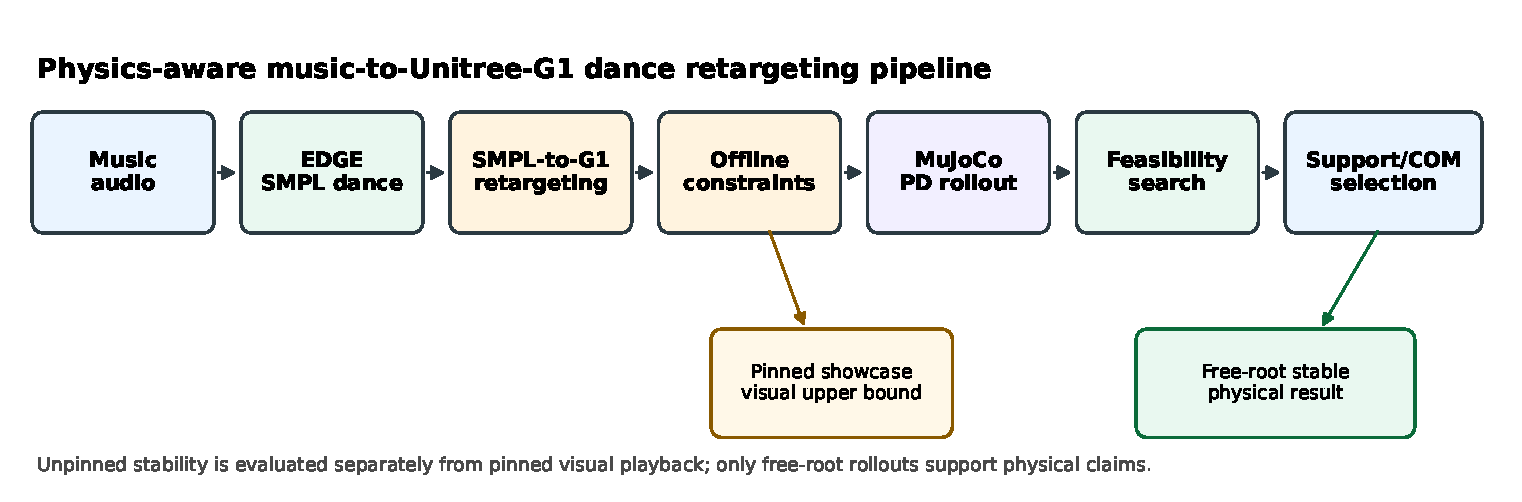
\includegraphics[width=\linewidth]{figures/pipeline_overview.pdf}
\caption{Final project pipeline. The system separates nonphysical pinned visualization from free-root simulation evaluation, so stability claims are limited to unpinned rollouts under the chosen MuJoCo model and PD controller.}
\label{fig:pipeline}
\end{figure}

\subsection{SMPL-to-G1 Retargeting}
The baseline retargeter maps SMPL joint rotations to corresponding G1 lower-body, waist, shoulder, elbow, and wrist joints after converting the SMPL human frame to MuJoCo's $z$-up frame. This direct mapping is useful as a diagnostic baseline because it keeps substantial human motion, but it frequently violates the balance assumptions of the robot. The improved v2 retargeter keeps the lower-body mapping and improves the arms with an inverse-kinematics-style method. SMPL forward kinematics gives target upper-arm and forearm directions. Each target upper-arm direction is expressed in the local G1 shoulder frame, shoulder pitch and roll are solved as a two-degree-of-freedom pointing problem, and elbow angle is set from the upper-arm--forearm angle. This improves upper-body visual correspondence without solving a full whole-body inverse kinematics problem.

\subsection{Offline Constraints and Contact Processing}
The offline constraint stage makes the retargeted reference more robot-friendly before simulation. It applies moving-average smoothing, rate limiting, acceleration limiting, root roll/pitch damping, joint-range clipping, and support-foot stabilization in detected contact segments. The constraints are body-part dependent: wrist motion is strongly damped, shoulder and elbow motion are preserved more for visual dance gestures, waist motion is reduced, and hip, knee, and ankle motions are kept conservative because they directly affect support and balance. The current implementation supports multiple profiles, including a safe profile for the main simulation-stability baseline, an expressive profile for preserving upper-body motion, a balance profile for stable free-root rollouts, and a showcase profile for pinned-root videos.

The final code also includes a contact-aware balance post-processor for the common case where a showcase reference looks good with root pinning but falls in free-root simulation. It estimates left and right foot contact intervals from foot height and speed, computes a support-center trajectory, damps risky lower-body and root motion, and applies a clipped PD-style correction to the floating-base horizontal trajectory. This module is not a full controller, but it provides a practical bridge between the visually expressive branch and the simulation-stable branch used in the final demos.

\section{Physics-Aware Optimization}
The first optimization stage searches for a feasible reference by scaling body-group motions. A candidate is parameterized as
\begin{equation}
\theta=(g_{\rm leg},g_{\rm arm},g_{\rm waist},g_{xy},g_{\psi},g_z,s),
\end{equation}
where the gains control lower-body amplitude, upper-body amplitude, waist motion, root translation, root yaw, vertical motion, and smoothing strength. For each candidate $q_\theta(t)$, an unpinned MuJoCo rollout computes stability rate $r_{\rm stab}$, minimum pelvis height $h_{\min}$, mean tracking error $e_{\rm track}$, and a motion amplitude score $m(q_\theta)$. The feasibility score is
\begin{align}
J_{\rm feas}(\theta)={}&w_f(1-r_{\rm stab})+w_h[h^*_{\min}-h_{\min}]_+ \nonumber\\
&+w_e e_{\rm track}-w_m m(q_\theta).
\end{align}
This lightweight rollout search is not full trajectory optimization, but it directly optimizes the main failure mode: early falls under free-root dynamics.

The final optimizer adds a heuristic support/center-of-mass proximity metric computed on candidate reference kinematics before rollout. Foot contacts are estimated from ankle-link height and speed. The support center $s_{xy}(t)$ is the horizontal position of the active support foot or the mean of both feet during double support. The whole-body center of mass $c_{xy}(t)$ is computed from MuJoCo body inertial positions and masses. The support error is
\begin{equation}
e_{\rm sup}(t)=\|c_{xy}(t)-s_{xy}(t)\|_2.
\end{equation}
The final selection score augments feasibility with the mean and 95th-percentile support errors,
\begin{equation}
J_{\rm final}=J_{\rm feas}+w_s\bar e_{\rm sup}+w_p[e_{\rm sup}^{95}-\epsilon]_+.
\end{equation}
This is not a full ZMP, capture-point, or dynamic support-polygon constraint, and it is not a feedback balance controller. It is a reference-level kinematic support proxy combined with an unpinned rollout filter, encouraging candidates whose mass distribution remains close to the estimated support region while still rewarding recovered dance motion.

\section{Experiments}
The main experiment uses a 10-second pop-style input clip. All method variants use the same generated SMPL motion so that differences are caused by retargeting and reference optimization rather than by music content. We compare five unpinned references: direct retargeting, offline-filtered retargeting, a conservative balance-safe baseline, the feasibility-optimized reference, and the final support/COM-aware reference. MuJoCo is simulated with a 0.002 s time step and PD position control over the 29 actuated G1 joints. A fall is declared when pelvis height drops below 0.35 m.

The reported metrics are stability rate, fall time, mean actuated joint tracking error, minimum pelvis height, and mean actuated joint motion amplitude. Stability rate is the fraction of the evaluated rollout before the pelvis crosses the fall threshold. Tracking error is the mean absolute error over actuated joint coordinates during PD rollout. Motion amplitude is the mean temporal standard deviation of actuated joint references, so it is a compact proxy for how much visible robot motion remains. Higher stability and amplitude are desirable, while lower tracking error is better, but amplitude should be interpreted relative to both the stable baseline and the unstable direct retargeting result. Beat alignment is computed only for the generated human motion using the EDGE-style acceleration-peak metric; the pop clip obtains a beat-alignment score of 0.6866 with 9 detected music beats and 62 motion beats. The current report does not claim robot-level beat alignment after retargeting, which remains a useful future metric. We additionally report a joint-limit boundary proxy for direct retargeting, defined as the fraction of hinge-joint frame entries that land within a small tolerance of a joint limit after clipping; this proxy is 0.69\% on the pop clip.

In addition to the quantitative MuJoCo rollouts, the final demonstrations are used as a qualitative comparison rather than as six separate case studies. These presentation videos are separate from the supplemental Jazz/Ballet-Jazz and Break metric exports: the numeric tables evaluate Pop plus two AIST-style stress checks, while the curated demo videos use Waack and Pop because they communicate the visual stability--expressiveness trade-off more clearly. The demos are organized around three conditions: pinned-root showcase playback, expressive free-root rollout, and stability-oriented free-root rollout. The pinned condition shows the visual upper range of the generated choreography but is nonphysical; the expressive free-root condition shows what happens when visual motion is retained too aggressively; and the stability-oriented free-root condition shows the result after contact-aware and support-oriented processing.

\begin{table}[t]
\centering
\caption{Final unpinned MuJoCo rollout results on the pop-style clip. Higher stability and amplitude are better; lower tracking error is better.}
\label{tab:final-results}
\setlength{\tabcolsep}{2.4pt}
\begin{tabular}{lccccc}
\toprule
Method & Stab. & Fall & Err. & Pelvis & Amp. \\
\midrule
Direct retarget & 11.8\% & 1.18s & 0.0681 & 0.084 & 0.1412 \\
Offline-filtered & 16.3\% & 1.63s & 0.0132 & 0.058 & 0.0798 \\
Balance-safe & 100.0\% & none & 0.0034 & 0.789 & 0.0143 \\
Feasibility-opt. & 100.0\% & none & 0.0065 & 0.788 & 0.0516 \\
Support/COM-aware & 100.0\% & none & 0.0076 & 0.788 & 0.0606 \\
\bottomrule
\end{tabular}
\end{table}

\begin{figure}[t]
\centering
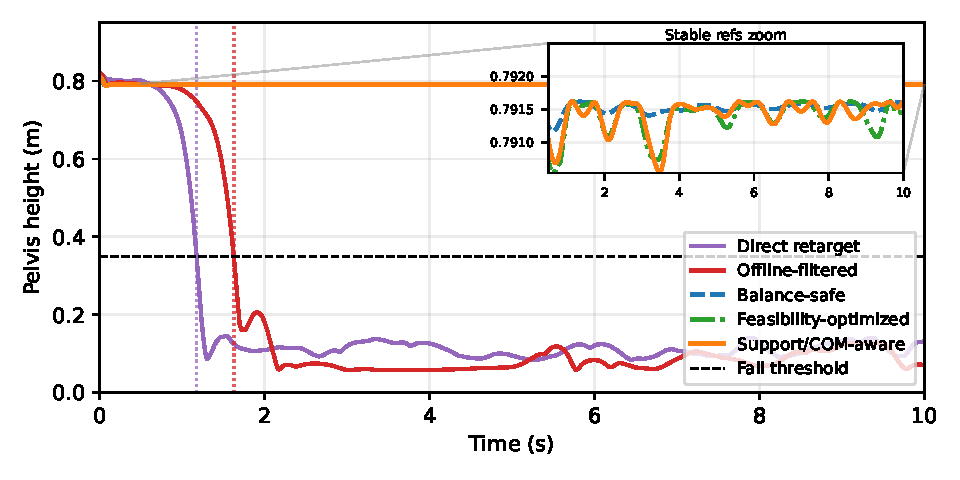
\includegraphics[width=\linewidth]{figures/final_stability_curve.pdf}
\caption{Pelvis height over time in unpinned MuJoCo rollouts. Direct retargeting and offline filtering fall early, while the conservative and optimized references remain above the fall threshold for the full rollout. The inset zooms the stable-reference region because the three stable curves nearly overlap around 0.79 m in the main plot.}
\label{fig:stability}
\end{figure}

To test whether the failure mode is specific to the pop example, we also evaluate two supplemental AIST-style motions. The Jazz/Ballet-Jazz example emphasizes upper-body motion, while the Break example is a harder stress test with sharper support and body-motion changes. These experiments are not a full multi-genre benchmark and should not be read as evidence of universal generalization across all music or dance styles, but they provide useful transfer checks. The supplemental metrics are evaluated over the available Jazz/Ballet-Jazz and Break sequences, which are 29.5 s and 48.0 s respectively; curated videos may show shorter demo excerpts. Each supplemental motion is processed through the same retargeting, conservative balance-safe baseline, feasibility optimization, and support/COM-aware optimization stages.

\begin{table}[t]
\centering
\caption{Supplemental cross-style checks. The final support/COM-aware reference remains stable in each style while recovering more motion than the balance-safe baseline.}
\label{tab:cross-style}
\setlength{\tabcolsep}{3pt}
\begin{tabular}{lcccc}
\toprule
Style & Direct fall & Final stab. & Safe amp. & Final amp. \\
\midrule
Pop-style & 1.18s & 100.0\% & 0.0143 & 0.0606 / 4.2$\times$ \\
Jazz/BJ & 0.78s & 100.0\% & 0.0228 & 0.0326 / 1.4$\times$ \\
Break & 1.02s & 100.0\% & 0.0156 & 0.0623 / 4.0$\times$ \\
\bottomrule
\end{tabular}
\end{table}

\begin{figure}[t]
\centering
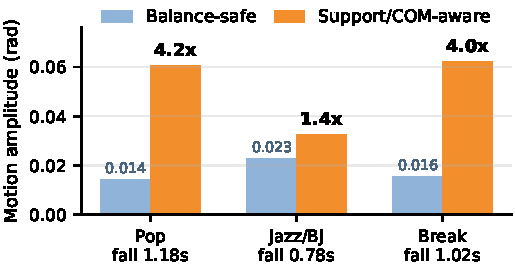
\includegraphics[width=\linewidth]{figures/cross_style_transfer.pdf}
\caption{Compact cross-style comparison for Pop, Jazz/Ballet-Jazz, and Break. Direct retargeting falls early, while support/COM-aware references remain stable and retain more motion than the conservative balance-safe baseline.}
\label{fig:cross-style}
\end{figure}

\section{Results and Discussion}
The pop-style results show the central stability--expressiveness trade-off. Direct retargeting preserves the most motion amplitude, but it falls after 1.18 s. Offline filtering reduces tracking error and removes joint-limit boundary issues, but it still falls after 1.63 s, showing that smoothing and clipping alone do not solve support and balance. The balance-safe baseline reaches 100\% stability, but its motion amplitude is only 0.0143, which makes the dance visually weak.

The feasibility optimizer also reaches 100\% stability while increasing amplitude to 0.0516. The final support/COM-aware reference remains stable and increases amplitude to 0.0606, which is about 4.2 times the conservative balance-safe amplitude but still only about 43\% of the unstable direct-retarget amplitude. This result supports the project hypothesis that reference-level physics awareness can recover meaningful dance motion without immediately requiring a learned controller, but it also shows that the current stable result comes mainly from strongly suppressing lower-body and root motion while preserving more upper-body expression. The selected pop support/COM parameters reflect this trade-off, with very small leg and root-translation gains and a larger arm gain. The supplemental checks show the same qualitative pattern: direct retargeting falls within approximately one second, while support/COM-aware references complete their evaluated Jazz/Ballet-Jazz (29.5 s) and Break (48.0 s) sequences without crossing the fall threshold. The Break example is particularly encouraging because the final amplitude is 0.0623, about 4.0 times its balance-safe baseline, but these checks remain stress tests rather than a full style-generalization benchmark.

The qualitative demonstrations further clarify the same trade-off across three conditions and two presentation styles, Waack and Pop. In the pinned-root showcase condition, both styles retain larger arm, torso, and root gestures, so they are the most visually dance-like, but this condition cannot support a physical stability claim because the floating base is artificially constrained. In the expressive free-root condition, the root is released while relatively large motion is preserved; this makes the limitation visible because an expressive Pop rollout can fall even though it looks closer to the generated human dance. In the stability-oriented free-root condition, both styles become more conservative after contact-aware and support-oriented processing, but the motions remain usable as simulation-stable references under the chosen MuJoCo model and PD controller. Waack is therefore used mainly as a strong visual showcase, while Pop connects the presentation videos to the main 10-second quantitative experiment. The Jazz/Ballet-Jazz and Break results should be read separately as supplemental stress checks on the same retargeting and optimization pipeline.

The remaining limitation is that the best unpinned simulation-stable motions are still less expressive than pinned-root showcase playback. This is expected because pinned playback removes the hardest part of the problem by forcing the floating base to follow the reference. The final demos therefore clearly separate pinned-root showcase videos from free-root stable videos. The former are nonphysical pinned visual references for dance expressiveness, while the latter provide the simulation-stability claim. Future work should replace the open-loop PD tracking assumption with a feedback balance controller, model-predictive control, or a learned tracking policy such as those used in physics-based humanoid control. Better lower-body inverse kinematics and explicit support-phase planning would also allow larger steps without destabilizing the robot.

\section{Conclusion}
This project implemented a working reference-level music-to-humanoid dance retargeting pipeline for Unitree G1 in MuJoCo. The experiments show that music-generated human dance is not directly simulation-stable for this floating-base humanoid setup: direct retargeting and offline filtering both fall quickly. By adding robot-specific constraints, rollout-based feasibility search, and support/COM-aware selection, the final system produces a 10-second free-root pop reference that is stable under the chosen MuJoCo model and PD controller, while preserving substantially more motion than a conservative stable baseline. The final contribution is therefore a physics-aware bridge between generative human dance and humanoid robot simulation, together with a quantitative analysis of the stability--expressiveness trade-off.

\section*{Author Contributions}
Zehui Liu led the overall system design and the main technical implementation of the project. Zehui implemented and integrated the music-conditioned G1 dance retargeting pipeline, including EDGE/SMPL motion processing, SMPL-to-G1 retargeting, MuJoCo PD rollout evaluation, offline physical constraints, balance-safe reference generation, rollout-based feasibility optimization, support/COM-aware selection, and the final evaluation scripts. Zehui also designed and executed the main Pop experiment and the supplemental Jazz/Ballet-Jazz and Break stress checks, generated and verified the final quantitative metrics, organized the final project structure, and prepared the final report package with figures, tables, references, selected videos, and code-polishing revisions.

Sijie Chen contributed to the repository setup and early project organization, and helped develop supporting components around the retargeting and evaluation workflow. Sijie's contributions included retargeting profile refinements, SMPL-to-reference comparison tools, contact-aware balance correction, presentation-oriented deliverables, curated comparison videos, and speaker-note materials. Sijie also contributed to qualitative demonstration design, especially the comparison between pinned-root visual showcases and free-root physical rollouts, and helped edit the report and presentation materials.

Both team members jointly contributed to the final problem formulation, experiment design, result interpretation, and final presentation narrative. In particular, both members discussed the stability--expressiveness trade-off, compared direct retargeting, offline filtering, conservative stable references, feasibility optimization, and support/COM-aware optimization, analyzed failure cases, and revised the final report to clearly separate nonphysical pinned-root visual references from free-root simulation-stability claims.

\bibliographystyle{plainnat}
\bibliography{references}

\end{CJK*}
\end{document}
